\documentclass[a4paper]{article}
\title{SmartFolder}
\author{Maxime Lovino \and Thomas Ibanez}
\usepackage[francais]{babel}
\usepackage{fontspec}
\usepackage{pgfplots}
\pgfplotsset{width=10cm,compat=1.9}
% \setmainfont{Helvetica Neue}
\usepackage{amsmath}
\usepackage{amsfonts}
\usepackage{xcolor,graphicx}
\definecolor{light-gray}{gray}{0.95}
\usepackage{minted}
\usemintedstyle{colorful}
\setlength{\parindent}{0pt}
\usepackage[left=2.5cm,top=2.5cm,right=2.5cm,bottom=2.5cm]{geometry}
\begin{document}
\maketitle
\newpage
\section{Introduction}
Hello world
\section{Architecture}
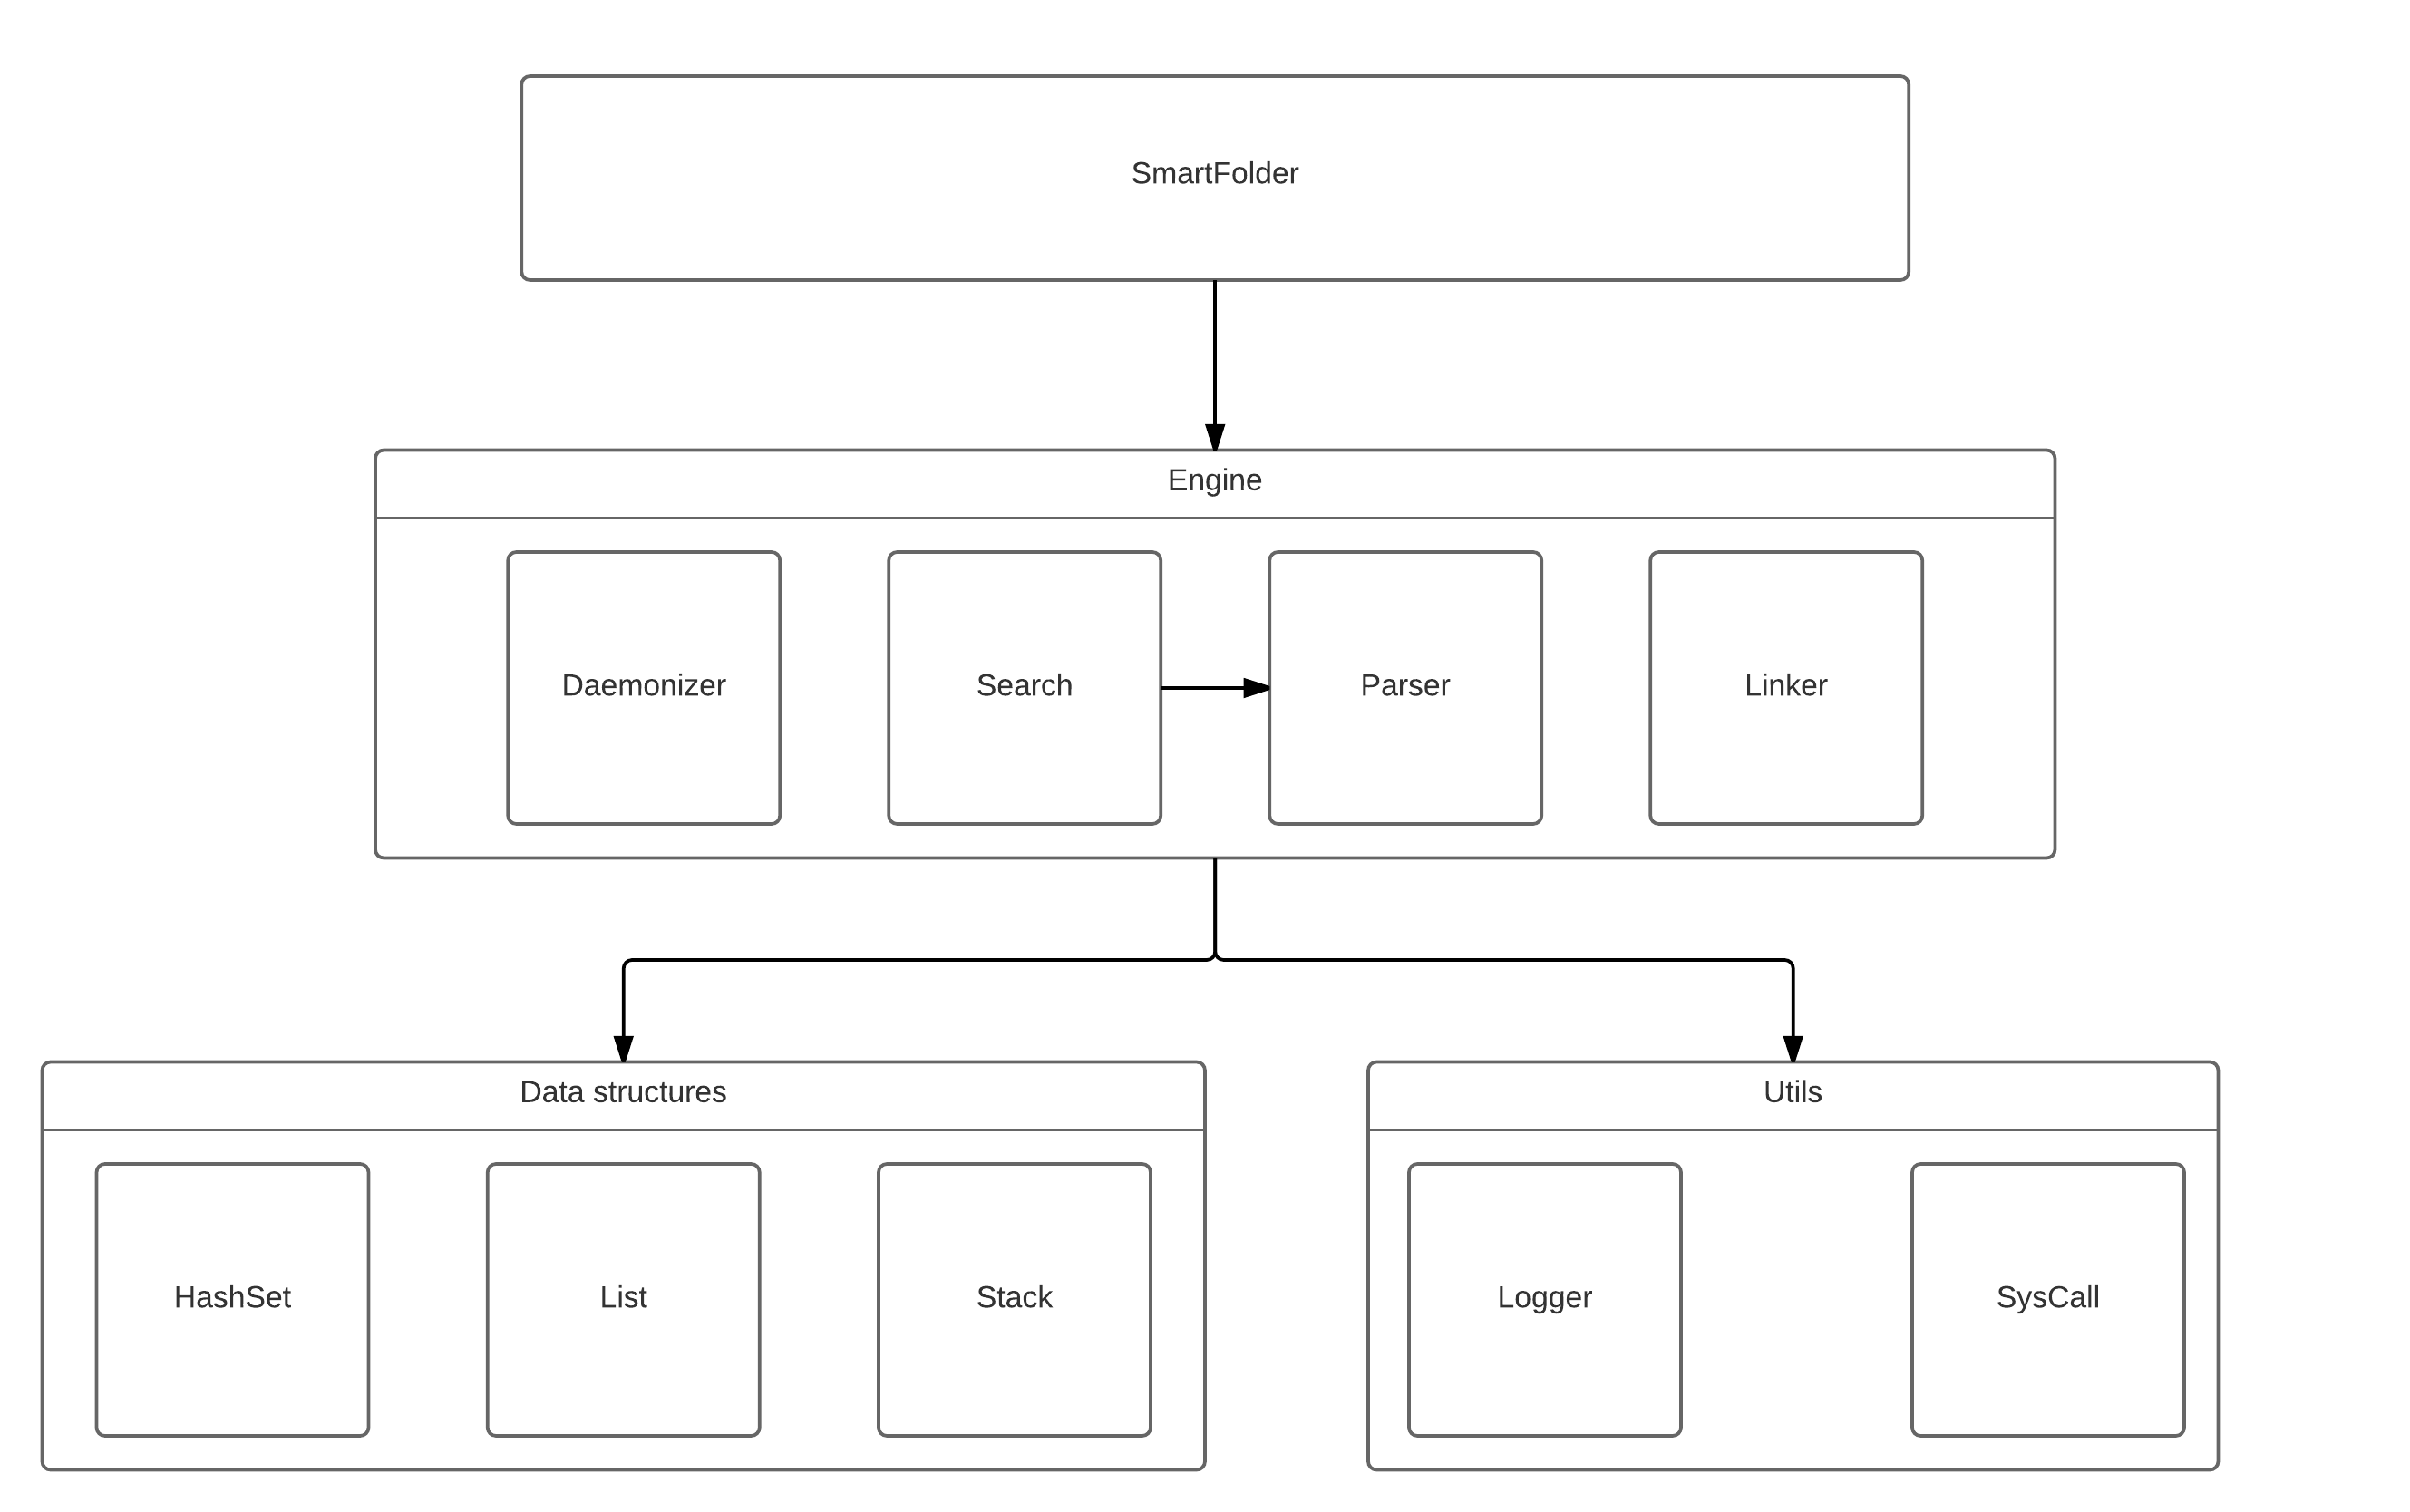
\includegraphics[width=\textwidth]{diagram.png}
\subsection{Data Structures}
\subsubsection{List}
Nous avons une structure de liste qui sert à stocker la liste des résultats d'une recherhe (liste de fichiers). Nous définissions des fonctions permettant d'agréer plusieurs listes au travers d'une union, intersection, etc... correspondant aux opérations booléennes classiques.
\subsubsection{HashSet}
Nous avons une structure de table de hachage permettant de stocker les matches actuels présent dans le dossier, cela nous permet lors du prochain run de la recherche de tester de façon rapide (recherche en $O(1)$ en général et maximum en $\Theta(n)$).
\subsubsection{Stack}
Nous utilisons une structure de Pile pour stocker les résultats d'une recherche particulière (on stocke un pointeur de la liste des résultats) pour ensuite les rassembler lorsque nous trouvons un opérateur booléen. (principe de l'évaluation d'une expression polonaise inverse)
\newpage
\subsection{Utils}
\subsubsection{Logger}
Nous avons réalisé un Logger pour pouvoir afficher sur la console des messages de notre programme, pour ceci nous définissons 3 niveaux de severité pour un message:
\begin{itemize}
	\item 0: INFO, un message d'information, par exemple un dump de hashtable ou des informations sur les fichiers trouvés
	\item 1: WARNING, un message de warning, par exemple une erreur dans notre programme durant son execution mais qui n'empêche pas le programme de continuer
	\item 2: FATAL, un message d'erreur, lorsqu'une erreur se produit qui fait crasher le programme entièrement
\end{itemize}
Dans le fichier \verb+Logger.h+ on peut changer la valeur du \verb+#define LOG_LEVEL X+ par le niveau minimal que l'on veut. C'est-à-dire que si nous définissons 1 ici, le logger affichera uniquement les messages de niveau 1 et 2. \\

Dans notre code nous pouvons utiliser la fonction \verb+void logMessage(int level, const char* format, ...);+ pour logger un message en spécifiant son niveau et en utilisant une syntaxe similaire à \verb+printf(...)+ ensuite.
\subsubsection{SysCall}
Nous avons un fichier regroupant des fonctions wrappers pour les appels systèmes que nous utilisons dans les différentes parties de notre programme. De ce fait, si nous voulons porter notre programme sur un autre système, nous avons juste à modifier le contenu de ces fonctions pour adapter ces appels systèmes.
\subsection{Engine}
\subsubsection{Search}
Dans la partie recherche nous avons la fonction qui va effectuer une recherche d'un certain type avec un certain argument de recherche dans un dossier et va retourner une liste des résultats de cette recherche. Nous définissons les types de recherche possible dans une énumération. Nous passons à la fonction le dossier à chercher, le type de recherche et l'argument de la recherche en question.
\subsubsection{Parser}
Ici nous avons la grande partie du programme, avec principalement la fonction
\begin{verbatim}
	int evaluateAndSearch(char** expression, int exprLen, char* folder, HashSet** result)
\end{verbatim}
qui va analyser la query passée en paramètre au programme (sous forme polonaise inverse) et l'éxecuter en stockant les résulats dans le HashSet \verb+result+.

Nous avons également d'autres fonctions permettant de vérifier si une fragment de recherche est valide, détecter des opérateurs booléens, recupérer l'UID d'un nom d'utilisateur ainsi que vérifier que le chemin d'accès du dossier est valide. Pour cette dernière, nous utilisons une RegExp en utilisant \verb+Regex.h+ pour computer la regex.
\subsubsection{Linker}
Le Linker sert à créer un lien symbolique vers un fichier dans le dossier de destination, il va s'occuper de créer un symlink avec le nom du fichier et gérer les collisions de noms le cas échéant (par exemple \verb+./a.txt+ et \verb+./abc/a.txt+ vont donner des symLink \verb+a.txt+ et \verb+a(1).txt+)
\subsubsection{Daemonizer}
Le Daemonizer va s'occuper de faire tourner en arrière-plan notre programme et de merger les nouveaux résultats de recherche avec les résultats déjà liés précedemment. Cela comprendra également la suppression de fichiers qui n'existent plus dans le dossier d'origine.
\subsection{SmartFolder}
Partie principale du programme, c'est ici qu'on s'occupera de prendre les arguments de l'utilisateur pour la création d'une instance de SmartFolder, ainsi que pour la suppression d'un SmartFolder existant.
\section{Utilisation du programme}
Nous pourrons appeler notre programme de deux manières, premièrement pour créer un SmartFolder:
\begin{verbatim}
SmartFolder <linkDirectory> <searchDir> [searchQuery]
\end{verbatim}
ou pour supprimer un SmartFolder existant:
\begin{verbatim}
	SmartFolder -d <linkDirectory>
\end{verbatim}
\subsection{Syntaxe de recherche}
Au niveau de la \verb+[searchQuery]+ les arguments suivant pourront être utilisés
\begin{itemize}
	\item \verb/--name <name>/
	\item \verb/--size [-+]<size>/
	\item \verb/--dateStatus [-+]<YYYY-MM-DD>/
	\item \verb/--dateModified [-+]<YYYY-MM-DD>/
	\item \verb/--dateUsed [-+]<YYYY-MM-DD>/
	\item \verb/--uid <loginName>/
	\item \verb/--gid <groupName>/
	\item \verb/--perms <octal>/
\end{itemize}
ainsi que les opérateurs booléens classiques sous cette forme
\begin{itemize}
	\item \verb+AND+
	\item \verb+OR+
	\item \verb+XOR+
	\item \verb+NOT+
\end{itemize}

La query sera sous la forme polonaise inverse, ce qui donne par exemple pour chercher tous les fichiers contenant \verb+toto+ dans le nom ET ayant comme permissions 777 OU les fichiers du user \verb+lovino+.
\begin{verbatim}
	--name toto --perms 777 AND --uid lovino OR
\end{verbatim}
\end{document}
